\documentclass[border=15pt]{standalone}
\usepackage{tikz}
\usepackage{xcolor}
\usetikzlibrary{positioning, fit, backgrounds, calc}

% ── Colors ──────────────────────────────────────────────────────────────────
\definecolor{coreFill}{HTML}{E3F2FD}
\definecolor{coreBorder}{HTML}{1565C0}
\definecolor{coreHeader}{HTML}{1565C0}

\definecolor{eventFill}{HTML}{FFF3E0}
\definecolor{eventBorder}{HTML}{E65100}
\definecolor{eventHeader}{HTML}{E65100}

\definecolor{payFill}{HTML}{FFF8E1}
\definecolor{payBorder}{HTML}{F57F17}
\definecolor{payHeader}{HTML}{F57F17}

\definecolor{commFill}{HTML}{E8F5E9}
\definecolor{commBorder}{HTML}{2E7D32}
\definecolor{commHeader}{HTML}{2E7D32}

\definecolor{notifFill}{HTML}{EDE7F6}
\definecolor{notifBorder}{HTML}{4527A0}
\definecolor{notifHeader}{HTML}{4527A0}

\definecolor{pkcolor}{HTML}{B71C1C}
\definecolor{fkcolor}{HTML}{1565C0}
\definecolor{rowtext}{HTML}{263238}

\begin{document}
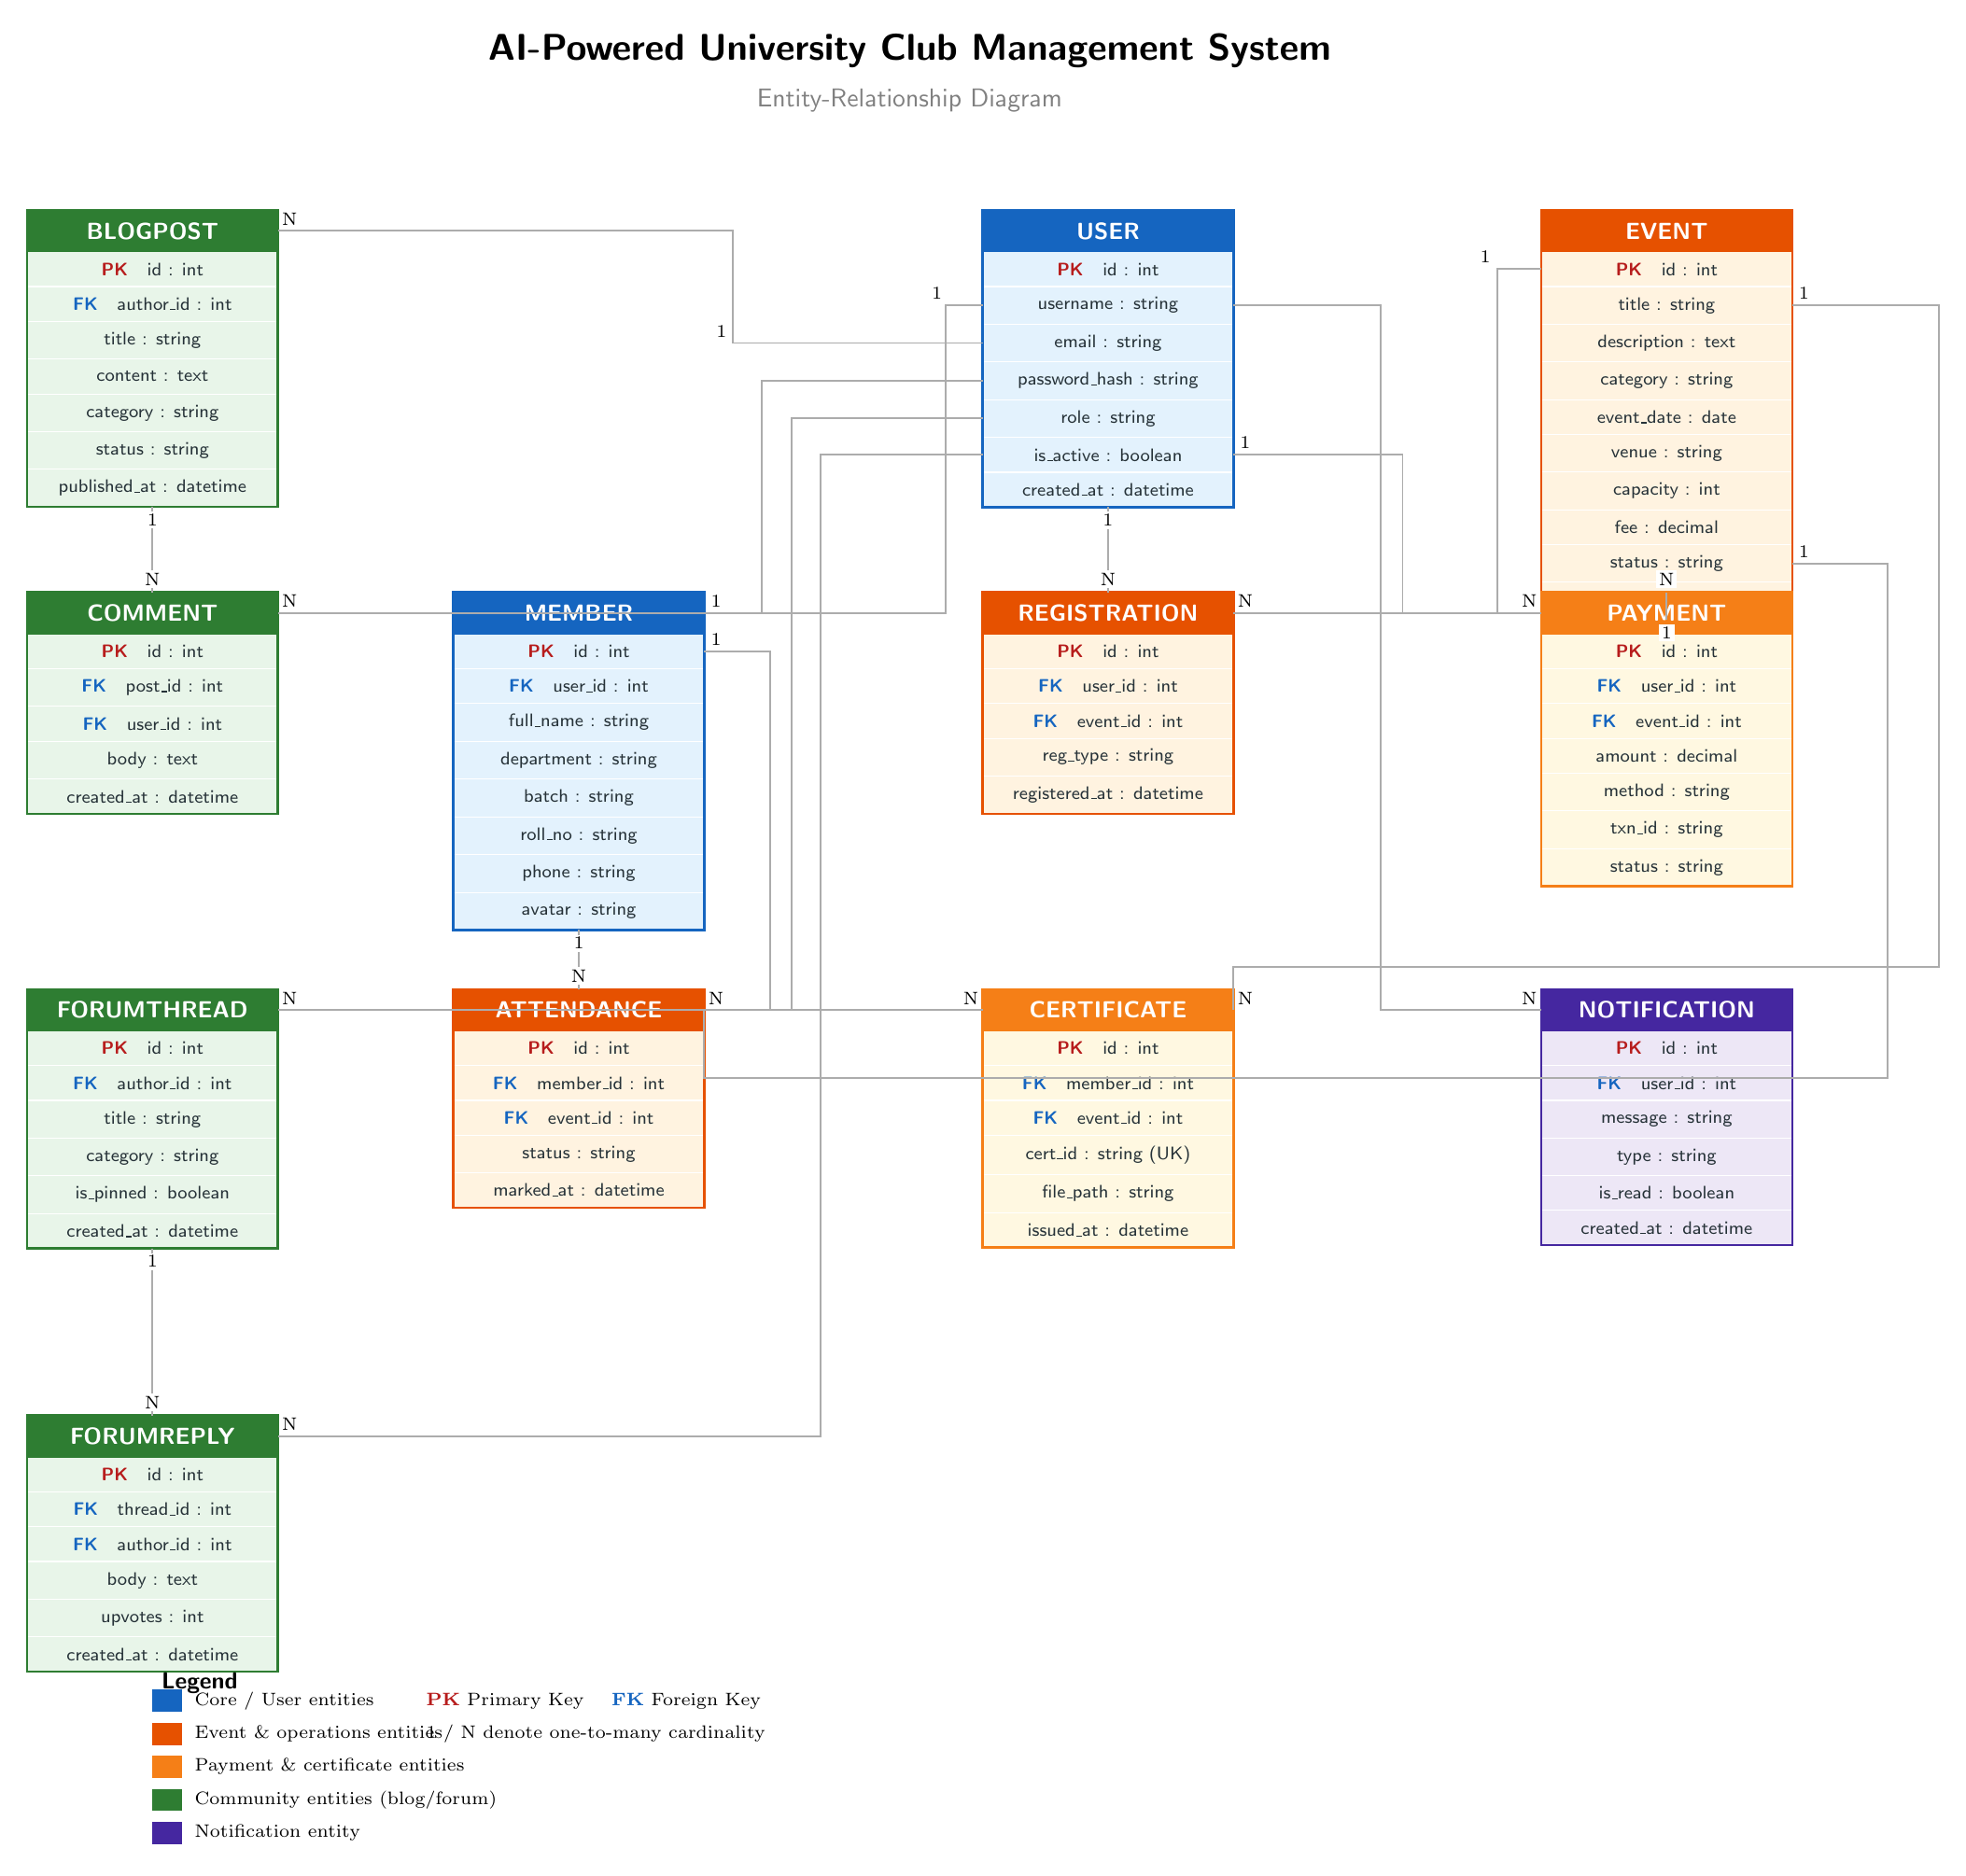
\begin{tikzpicture}[
  font=\sffamily,
  every node/.style={font=\sffamily},
  scale=1, transform shape
]

% ──────────────────────────────────────────────────────────────────────────
% Macro to draw an entity table
% #1 = node name, #2 = x, #3 = y, #4 = title, #5 = header color, #6 = fill color, #7 = border color, #8 = rows (list of "PK/FK & name & type")
% ──────────────────────────────────────────────────────────────────────────

\newcommand{\entitytable}[6]{%
  % #1=name #2=x #3=y #4=title #5=headercolor #6=rows(macro)
}

% Helper to build a table manually using matrix-like nodes
\tikzset{
  ent header/.style={
    rectangle, minimum width=3.4cm, minimum height=0.55cm,
    fill=#1, text=white, font=\sffamily\bfseries\small, align=center
  },
  ent row/.style={
    rectangle, minimum width=3.4cm, minimum height=0.46cm,
    fill=#1, text=rowtext, font=\sffamily\scriptsize, align=left, inner sep=4pt
  }
}

% ════════════════════════════════════════════════════════════════════════
% ENTITY: USER  (core, blue)
% ════════════════════════════════════════════════════════════════════════
\begin{scope}[local bounding box=USER]
\node[ent header=coreHeader] (user-h) at (0,10) {USER};
\node[ent row=coreFill, anchor=north] (user-r1) at (user-h.south) {\textcolor{pkcolor}{\bfseries PK} ~ id : int};
\node[ent row=coreFill, anchor=north] (user-r2) at (user-r1.south) {username : string};
\node[ent row=coreFill, anchor=north] (user-r3) at (user-r2.south) {email : string};
\node[ent row=coreFill, anchor=north] (user-r4) at (user-r3.south) {password\_hash : string};
\node[ent row=coreFill, anchor=north] (user-r5) at (user-r4.south) {role : string};
\node[ent row=coreFill, anchor=north] (user-r6) at (user-r5.south) {is\_active : boolean};
\node[ent row=coreFill, anchor=north] (user-r7) at (user-r6.south) {created\_at : datetime};
\draw[coreBorder, line width=0.9pt] (user-h.north west) rectangle (user-r7.south east);
\draw[coreBorder, line width=0.6pt] (user-h.south west) -- (user-h.south east);
\end{scope}

% ════════════════════════════════════════════════════════════════════════
% ENTITY: MEMBER (core, blue)
% ════════════════════════════════════════════════════════════════════════
\node[ent header=coreHeader] (mem-h) at (-7.2,4.8) {MEMBER};
\node[ent row=coreFill, anchor=north] (mem-r1) at (mem-h.south) {\textcolor{pkcolor}{\bfseries PK} ~ id : int};
\node[ent row=coreFill, anchor=north] (mem-r2) at (mem-r1.south) {\textcolor{fkcolor}{\bfseries FK} ~ user\_id : int};
\node[ent row=coreFill, anchor=north] (mem-r3) at (mem-r2.south) {full\_name : string};
\node[ent row=coreFill, anchor=north] (mem-r4) at (mem-r3.south) {department : string};
\node[ent row=coreFill, anchor=north] (mem-r5) at (mem-r4.south) {batch : string};
\node[ent row=coreFill, anchor=north] (mem-r6) at (mem-r5.south) {roll\_no : string};
\node[ent row=coreFill, anchor=north] (mem-r7) at (mem-r6.south) {phone : string};
\node[ent row=coreFill, anchor=north] (mem-r8) at (mem-r7.south) {avatar : string};
\draw[coreBorder, line width=0.9pt] (mem-h.north west) rectangle (mem-r8.south east);
\draw[coreBorder, line width=0.6pt] (mem-h.south west) -- (mem-h.south east);

% ════════════════════════════════════════════════════════════════════════
% ENTITY: EVENT (event, orange)
% ════════════════════════════════════════════════════════════════════════
\node[ent header=eventHeader] (ev-h) at (7.6,10) {EVENT};
\node[ent row=eventFill, anchor=north] (ev-r1) at (ev-h.south) {\textcolor{pkcolor}{\bfseries PK} ~ id : int};
\node[ent row=eventFill, anchor=north] (ev-r2) at (ev-r1.south) {title : string};
\node[ent row=eventFill, anchor=north] (ev-r3) at (ev-r2.south) {description : text};
\node[ent row=eventFill, anchor=north] (ev-r4) at (ev-r3.south) {category : string};
\node[ent row=eventFill, anchor=north] (ev-r5) at (ev-r4.south) {event\_date : date};
\node[ent row=eventFill, anchor=north] (ev-r6) at (ev-r5.south) {venue : string};
\node[ent row=eventFill, anchor=north] (ev-r7) at (ev-r6.south) {capacity : int};
\node[ent row=eventFill, anchor=north] (ev-r8) at (ev-r7.south) {fee : decimal};
\node[ent row=eventFill, anchor=north] (ev-r9) at (ev-r8.south) {status : string};
\node[ent row=eventFill, anchor=north] (ev-r10) at (ev-r9.south) {is\_public : boolean};
\draw[eventBorder, line width=0.9pt] (ev-h.north west) rectangle (ev-r10.south east);
\draw[eventBorder, line width=0.6pt] (ev-h.south west) -- (ev-h.south east);

% ════════════════════════════════════════════════════════════════════════
% ENTITY: REGISTRATION (event, orange)
% ════════════════════════════════════════════════════════════════════════
\node[ent header=eventHeader] (reg-h) at (0,4.8) {REGISTRATION};
\node[ent row=eventFill, anchor=north] (reg-r1) at (reg-h.south) {\textcolor{pkcolor}{\bfseries PK} ~ id : int};
\node[ent row=eventFill, anchor=north] (reg-r2) at (reg-r1.south) {\textcolor{fkcolor}{\bfseries FK} ~ user\_id : int};
\node[ent row=eventFill, anchor=north] (reg-r3) at (reg-r2.south) {\textcolor{fkcolor}{\bfseries FK} ~ event\_id : int};
\node[ent row=eventFill, anchor=north] (reg-r4) at (reg-r3.south) {reg\_type : string};
\node[ent row=eventFill, anchor=north] (reg-r5) at (reg-r4.south) {registered\_at : datetime};
\draw[eventBorder, line width=0.9pt] (reg-h.north west) rectangle (reg-r5.south east);
\draw[eventBorder, line width=0.6pt] (reg-h.south west) -- (reg-h.south east);

% ════════════════════════════════════════════════════════════════════════
% ENTITY: ATTENDANCE (event, orange)
% ════════════════════════════════════════════════════════════════════════
\node[ent header=eventHeader] (att-h) at (-7.2,-0.6) {ATTENDANCE};
\node[ent row=eventFill, anchor=north] (att-r1) at (att-h.south) {\textcolor{pkcolor}{\bfseries PK} ~ id : int};
\node[ent row=eventFill, anchor=north] (att-r2) at (att-r1.south) {\textcolor{fkcolor}{\bfseries FK} ~ member\_id : int};
\node[ent row=eventFill, anchor=north] (att-r3) at (att-r2.south) {\textcolor{fkcolor}{\bfseries FK} ~ event\_id : int};
\node[ent row=eventFill, anchor=north] (att-r4) at (att-r3.south) {status : string};
\node[ent row=eventFill, anchor=north] (att-r5) at (att-r4.south) {marked\_at : datetime};
\draw[eventBorder, line width=0.9pt] (att-h.north west) rectangle (att-r5.south east);
\draw[eventBorder, line width=0.6pt] (att-h.south west) -- (att-h.south east);

% ════════════════════════════════════════════════════════════════════════
% ENTITY: PAYMENT (payment, gold)
% ════════════════════════════════════════════════════════════════════════
\node[ent header=payHeader] (pay-h) at (7.6,4.8) {PAYMENT};
\node[ent row=payFill, anchor=north] (pay-r1) at (pay-h.south) {\textcolor{pkcolor}{\bfseries PK} ~ id : int};
\node[ent row=payFill, anchor=north] (pay-r2) at (pay-r1.south) {\textcolor{fkcolor}{\bfseries FK} ~ user\_id : int};
\node[ent row=payFill, anchor=north] (pay-r3) at (pay-r2.south) {\textcolor{fkcolor}{\bfseries FK} ~ event\_id : int};
\node[ent row=payFill, anchor=north] (pay-r4) at (pay-r3.south) {amount : decimal};
\node[ent row=payFill, anchor=north] (pay-r5) at (pay-r4.south) {method : string};
\node[ent row=payFill, anchor=north] (pay-r6) at (pay-r5.south) {txn\_id : string};
\node[ent row=payFill, anchor=north] (pay-r7) at (pay-r6.south) {status : string};
\draw[payBorder, line width=0.9pt] (pay-h.north west) rectangle (pay-r7.south east);
\draw[payBorder, line width=0.6pt] (pay-h.south west) -- (pay-h.south east);

% ════════════════════════════════════════════════════════════════════════
% ENTITY: CERTIFICATE (payment, gold)
% ════════════════════════════════════════════════════════════════════════
\node[ent header=payHeader] (cert-h) at (0,-0.6) {CERTIFICATE};
\node[ent row=payFill, anchor=north] (cert-r1) at (cert-h.south) {\textcolor{pkcolor}{\bfseries PK} ~ id : int};
\node[ent row=payFill, anchor=north] (cert-r2) at (cert-r1.south) {\textcolor{fkcolor}{\bfseries FK} ~ member\_id : int};
\node[ent row=payFill, anchor=north] (cert-r3) at (cert-r2.south) {\textcolor{fkcolor}{\bfseries FK} ~ event\_id : int};
\node[ent row=payFill, anchor=north] (cert-r4) at (cert-r3.south) {cert\_id : string (UK)};
\node[ent row=payFill, anchor=north] (cert-r5) at (cert-r4.south) {file\_path : string};
\node[ent row=payFill, anchor=north] (cert-r6) at (cert-r5.south) {issued\_at : datetime};
\draw[payBorder, line width=0.9pt] (cert-h.north west) rectangle (cert-r6.south east);
\draw[payBorder, line width=0.6pt] (cert-h.south west) -- (cert-h.south east);

% ════════════════════════════════════════════════════════════════════════
% ENTITY: BLOGPOST (community, green)
% ════════════════════════════════════════════════════════════════════════
\node[ent header=commHeader] (blog-h) at (-13,10) {BLOGPOST};
\node[ent row=commFill, anchor=north] (blog-r1) at (blog-h.south) {\textcolor{pkcolor}{\bfseries PK} ~ id : int};
\node[ent row=commFill, anchor=north] (blog-r2) at (blog-r1.south) {\textcolor{fkcolor}{\bfseries FK} ~ author\_id : int};
\node[ent row=commFill, anchor=north] (blog-r3) at (blog-r2.south) {title : string};
\node[ent row=commFill, anchor=north] (blog-r4) at (blog-r3.south) {content : text};
\node[ent row=commFill, anchor=north] (blog-r5) at (blog-r4.south) {category : string};
\node[ent row=commFill, anchor=north] (blog-r6) at (blog-r5.south) {status : string};
\node[ent row=commFill, anchor=north] (blog-r7) at (blog-r6.south) {published\_at : datetime};
\draw[commBorder, line width=0.9pt] (blog-h.north west) rectangle (blog-r7.south east);
\draw[commBorder, line width=0.6pt] (blog-h.south west) -- (blog-h.south east);

% ════════════════════════════════════════════════════════════════════════
% ENTITY: COMMENT (community, green)
% ════════════════════════════════════════════════════════════════════════
\node[ent header=commHeader] (com-h) at (-13,4.8) {COMMENT};
\node[ent row=commFill, anchor=north] (com-r1) at (com-h.south) {\textcolor{pkcolor}{\bfseries PK} ~ id : int};
\node[ent row=commFill, anchor=north] (com-r2) at (com-r1.south) {\textcolor{fkcolor}{\bfseries FK} ~ post\_id : int};
\node[ent row=commFill, anchor=north] (com-r3) at (com-r2.south) {\textcolor{fkcolor}{\bfseries FK} ~ user\_id : int};
\node[ent row=commFill, anchor=north] (com-r4) at (com-r3.south) {body : text};
\node[ent row=commFill, anchor=north] (com-r5) at (com-r4.south) {created\_at : datetime};
\draw[commBorder, line width=0.9pt] (com-h.north west) rectangle (com-r5.south east);
\draw[commBorder, line width=0.6pt] (com-h.south west) -- (com-h.south east);

% ════════════════════════════════════════════════════════════════════════
% ENTITY: FORUMTHREAD (community, green)
% ════════════════════════════════════════════════════════════════════════
\node[ent header=commHeader] (th-h) at (-13,-0.6) {FORUMTHREAD};
\node[ent row=commFill, anchor=north] (th-r1) at (th-h.south) {\textcolor{pkcolor}{\bfseries PK} ~ id : int};
\node[ent row=commFill, anchor=north] (th-r2) at (th-r1.south) {\textcolor{fkcolor}{\bfseries FK} ~ author\_id : int};
\node[ent row=commFill, anchor=north] (th-r3) at (th-r2.south) {title : string};
\node[ent row=commFill, anchor=north] (th-r4) at (th-r3.south) {category : string};
\node[ent row=commFill, anchor=north] (th-r5) at (th-r4.south) {is\_pinned : boolean};
\node[ent row=commFill, anchor=north] (th-r6) at (th-r5.south) {created\_at : datetime};
\draw[commBorder, line width=0.9pt] (th-h.north west) rectangle (th-r6.south east);
\draw[commBorder, line width=0.6pt] (th-h.south west) -- (th-h.south east);

% ════════════════════════════════════════════════════════════════════════
% ENTITY: FORUMREPLY (community, green)
% ════════════════════════════════════════════════════════════════════════
\node[ent header=commHeader] (rep-h) at (-13,-6.4) {FORUMREPLY};
\node[ent row=commFill, anchor=north] (rep-r1) at (rep-h.south) {\textcolor{pkcolor}{\bfseries PK} ~ id : int};
\node[ent row=commFill, anchor=north] (rep-r2) at (rep-r1.south) {\textcolor{fkcolor}{\bfseries FK} ~ thread\_id : int};
\node[ent row=commFill, anchor=north] (rep-r3) at (rep-r2.south) {\textcolor{fkcolor}{\bfseries FK} ~ author\_id : int};
\node[ent row=commFill, anchor=north] (rep-r4) at (rep-r3.south) {body : text};
\node[ent row=commFill, anchor=north] (rep-r5) at (rep-r4.south) {upvotes : int};
\node[ent row=commFill, anchor=north] (rep-r6) at (rep-r5.south) {created\_at : datetime};
\draw[commBorder, line width=0.9pt] (rep-h.north west) rectangle (rep-r6.south east);
\draw[commBorder, line width=0.6pt] (rep-h.south west) -- (rep-h.south east);

% ════════════════════════════════════════════════════════════════════════
% ENTITY: NOTIFICATION (notif, purple)
% ════════════════════════════════════════════════════════════════════════
\node[ent header=notifHeader] (not-h) at (7.6,-0.6) {NOTIFICATION};
\node[ent row=notifFill, anchor=north] (not-r1) at (not-h.south) {\textcolor{pkcolor}{\bfseries PK} ~ id : int};
\node[ent row=notifFill, anchor=north] (not-r2) at (not-r1.south) {\textcolor{fkcolor}{\bfseries FK} ~ user\_id : int};
\node[ent row=notifFill, anchor=north] (not-r3) at (not-r2.south) {message : string};
\node[ent row=notifFill, anchor=north] (not-r4) at (not-r3.south) {type : string};
\node[ent row=notifFill, anchor=north] (not-r5) at (not-r4.south) {is\_read : boolean};
\node[ent row=notifFill, anchor=north] (not-r6) at (not-r5.south) {created\_at : datetime};
\draw[notifBorder, line width=0.9pt] (not-h.north west) rectangle (not-r6.south east);
\draw[notifBorder, line width=0.6pt] (not-h.south west) -- (not-h.south east);

% ════════════════════════════════════════════════════════════════════════
% RELATIONSHIPS  (1 ── N style labels, routed around tables, not through them)
% ════════════════════════════════════════════════════════════════════════
\begin{scope}[every path/.style={line width=0.7pt, draw=gray!65}]

% USER -> MEMBER (1:1)  -- short direct link, left side
\draw (user-r2.west) -- ++(-0.5,0) |- (mem-h.east);
\node[font=\scriptsize, fill=white, inner sep=1pt] at ($(user-r2.west)+(-0.62,0.16)$) {1};
\node[font=\scriptsize, fill=white, inner sep=1pt] at ($(mem-h.east)+(0.16,0.16)$) {1};

% USER -> REGISTRATION (1:N) -- straight down
\draw (user-r7.south) -- (reg-h.north);
\node[font=\scriptsize, fill=white, inner sep=1pt] at ($(user-r7.south)+(0,-0.18)$) {1};
\node[font=\scriptsize, fill=white, inner sep=1pt] at ($(reg-h.north)+(0,0.18)$) {N};

% USER -> PAYMENT (1:N) -- routed right, below EVENT, above PAYMENT
\draw (user-r6.east) -- ++(2.3,0) |- (pay-h.west);
\node[font=\scriptsize, fill=white, inner sep=1pt] at ($(user-r6.east)+(0.16,0.16)$) {1};
\node[font=\scriptsize, fill=white, inner sep=1pt] at ($(pay-h.west)+(-0.16,0.16)$) {N};

% USER -> BLOGPOST (1:N) -- routed left, above MEMBER
\draw (user-r3.west) -- ++(-3.4,0) |- (blog-h.east);
\node[font=\scriptsize, fill=white, inner sep=1pt] at ($(user-r3.west)+(-3.55,0.16)$) {1};
\node[font=\scriptsize, fill=white, inner sep=1pt] at ($(blog-h.east)+(0.16,0.16)$) {N};

% USER -> COMMENT (1:N) -- routed further left, below BLOGPOST link
\draw (user-r4.west) -- ++(-3.0,0) |- (com-h.east);
\node[font=\scriptsize, fill=white, inner sep=1pt] at ($(com-h.east)+(0.16,0.16)$) {N};

% USER -> FORUMTHREAD (1:N) -- routed left, lower
\draw (user-r5.west) -- ++(-2.6,0) |- (th-h.east);
\node[font=\scriptsize, fill=white, inner sep=1pt] at ($(th-h.east)+(0.16,0.16)$) {N};

% USER -> FORUMREPLY (1:N) -- routed left, lowest
\draw (user-r6.west) -- ++(-2.2,0) |- (rep-h.east);
\node[font=\scriptsize, fill=white, inner sep=1pt] at ($(rep-h.east)+(0.16,0.16)$) {N};

% USER -> NOTIFICATION (1:N) -- routed right, lower than PAYMENT
\draw (user-r2.east) -- ++(2.0,0) |- (not-h.west);
\node[font=\scriptsize, fill=white, inner sep=1pt] at ($(not-h.west)+(-0.16,0.16)$) {N};

% MEMBER -> ATTENDANCE (1:N) -- straight down
\draw (mem-r8.south) -- (att-h.north);
\node[font=\scriptsize, fill=white, inner sep=1pt] at ($(mem-r8.south)+(0,-0.18)$) {1};
\node[font=\scriptsize, fill=white, inner sep=1pt] at ($(att-h.north)+(0,0.18)$) {N};

% MEMBER -> CERTIFICATE (1:N) -- routed right below REGISTRATION
\draw (mem-r1.east) -- ++(0.9,0) |- (cert-h.west);
\node[font=\scriptsize, fill=white, inner sep=1pt] at ($(mem-r1.east)+(0.16,0.16)$) {1};
\node[font=\scriptsize, fill=white, inner sep=1pt] at ($(cert-h.west)+(-0.16,0.16)$) {N};

% EVENT -> REGISTRATION (1:N) -- routed left
\draw (ev-r1.west) -- ++(-0.6,0) |- (reg-h.east);
\node[font=\scriptsize, fill=white, inner sep=1pt] at ($(ev-r1.west)+(-0.76,0.16)$) {1};
\node[font=\scriptsize, fill=white, inner sep=1pt] at ($(reg-h.east)+(0.16,0.16)$) {N};

% EVENT -> ATTENDANCE (1:N) -- routed far right then down then left
\draw (ev-r9.east) -- ++(1.3,0) |- ++(0,-7.0) -| (att-h.east);
\node[font=\scriptsize, fill=white, inner sep=1pt] at ($(ev-r9.east)+(0.16,0.16)$) {1};
\node[font=\scriptsize, fill=white, inner sep=1pt] at ($(att-h.east)+(0.16,0.16)$) {N};

% EVENT -> PAYMENT (1:N) -- straight down
\draw (ev-r10.south) -- (pay-h.north);
\node[font=\scriptsize, fill=white, inner sep=1pt] at ($(ev-r10.south)+(0,-0.18)$) {1};
\node[font=\scriptsize, fill=white, inner sep=1pt] at ($(pay-h.north)+(0,0.18)$) {N};

% EVENT -> CERTIFICATE (1:N) -- routed right, down, then left into cert
\draw (ev-r2.east) -- ++(2.0,0) |- ++(0,-9.0) -| (cert-h.east);
\node[font=\scriptsize, fill=white, inner sep=1pt] at ($(ev-r2.east)+(0.16,0.16)$) {1};
\node[font=\scriptsize, fill=white, inner sep=1pt] at ($(cert-h.east)+(0.16,0.16)$) {N};

% BLOGPOST -> COMMENT (1:N) -- straight down
\draw (blog-r7.south) -- (com-h.north);
\node[font=\scriptsize, fill=white, inner sep=1pt] at ($(blog-r7.south)+(0,-0.18)$) {1};
\node[font=\scriptsize, fill=white, inner sep=1pt] at ($(com-h.north)+(0,0.18)$) {N};

% FORUMTHREAD -> FORUMREPLY (1:N) -- straight down
\draw (th-r6.south) -- (rep-h.north);
\node[font=\scriptsize, fill=white, inner sep=1pt] at ($(th-r6.south)+(0,-0.18)$) {1};
\node[font=\scriptsize, fill=white, inner sep=1pt] at ($(rep-h.north)+(0,0.18)$) {N};

\end{scope}

% ════════════════════════════════════════════════════════════════════════
% LEGEND
% ════════════════════════════════════════════════════════════════════════
\begin{scope}[shift={(-13,-9.5)}]
\node[anchor=north west, font=\sffamily\bfseries\small] at (0,0) {Legend};
\node[ent header=coreHeader, minimum width=0.4cm, minimum height=0.3cm] (lg1) at (0.2,-0.5) {};
\node[anchor=west, font=\scriptsize] at (0.45,-0.5) {Core / User entities};
\node[ent header=eventHeader, minimum width=0.4cm, minimum height=0.3cm] (lg2) at (0.2,-0.95) {};
\node[anchor=west, font=\scriptsize] at (0.45,-0.95) {Event \& operations entities};
\node[ent header=payHeader, minimum width=0.4cm, minimum height=0.3cm] (lg3) at (0.2,-1.4) {};
\node[anchor=west, font=\scriptsize] at (0.45,-1.4) {Payment \& certificate entities};
\node[anchor=west, font=\scriptsize] at (3.6,-0.5) {\textcolor{pkcolor}{\bfseries PK} Primary Key \quad \textcolor{fkcolor}{\bfseries FK} Foreign Key};
\node[ent header=commHeader, minimum width=0.4cm, minimum height=0.3cm] (lg4) at (0.2,-1.85) {};
\node[anchor=west, font=\scriptsize] at (0.45,-1.85) {Community entities (blog/forum)};
\node[ent header=notifHeader, minimum width=0.4cm, minimum height=0.3cm] (lg5) at (0.2,-2.3) {};
\node[anchor=west, font=\scriptsize] at (0.45,-2.3) {Notification entity};
\node[anchor=west, font=\scriptsize] at (3.6,-0.95) {1 / N denote one-to-many cardinality};
\end{scope}

% Title
\node[anchor=south, font=\sffamily\bfseries\Large] at (-2.7,12.1) {AI-Powered University Club Management System};
\node[anchor=south, font=\sffamily, gray] at (-2.7,11.5) {Entity-Relationship Diagram};

\end{tikzpicture}
\end{document}
